\begin{frame}{Voronoi Diagrams}
	\begin{itemize}
		\item The original set of points are now called \textbf{sites}
		\item Divide the plane into \textbf{regions of proximity}
		\item Consists of Voronoi edges and Voronoi vertices
		\item Useful to quickly find the nearest site for any given point in the plane

	\end{itemize}
	\begin{figure}
		\centering
		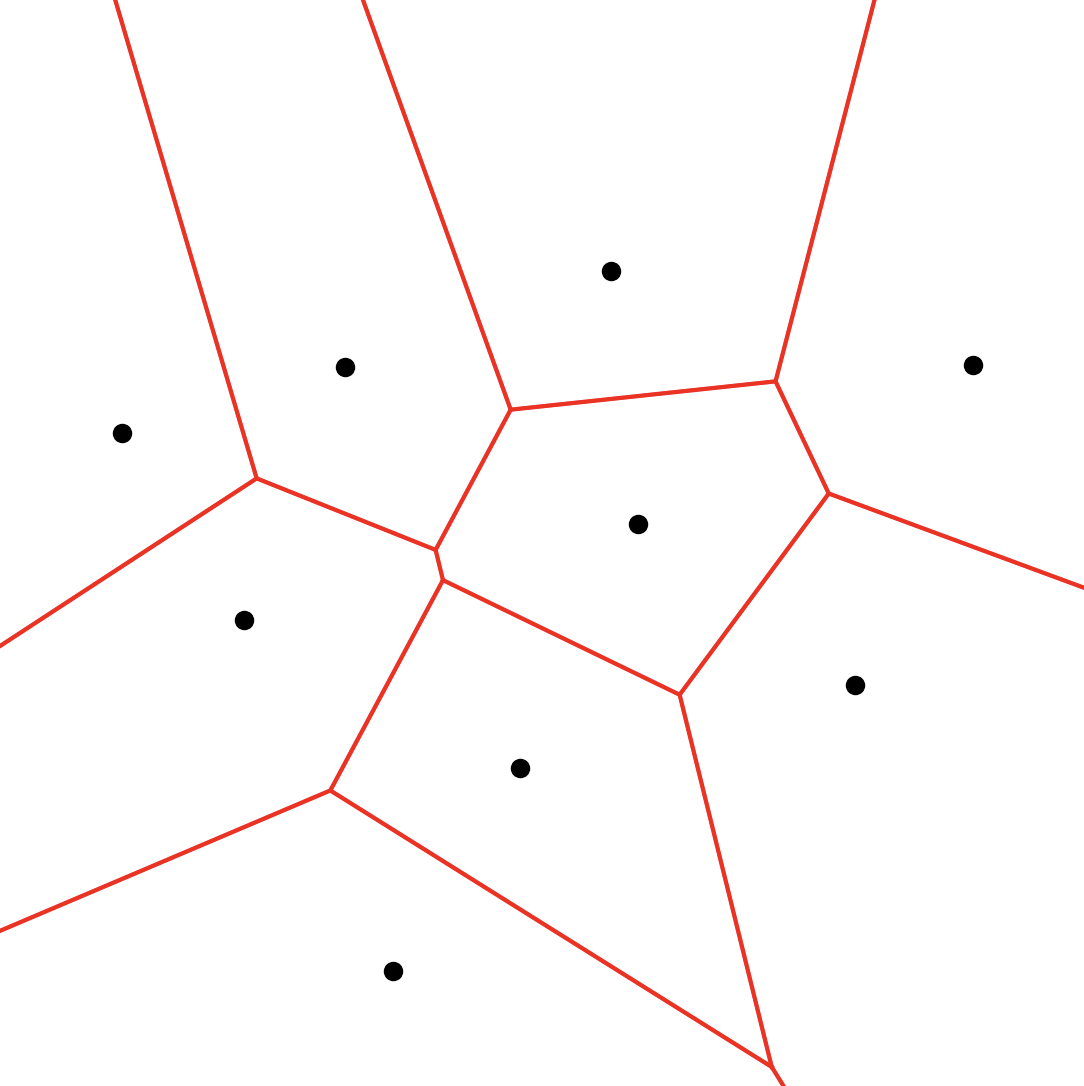
\includegraphics[width=0.4\textwidth]{figure_source/voronoi_diagram.png}
	\end{figure}
\end{frame}
